% Metódy inžinierskej práce

\documentclass[10pt,slovak,twoside,a4paper]{article}

\usepackage[slovak]{babel}
\usepackage[a4paper,inner=1.7cm, outer=2.7cm, top=2cm, bottom=2cm, bindingoffset=1.2cm]{geometry}
\usepackage{graphics}

\usepackage{cite}
%\usepackage{times}

\pagestyle{headings} 
%

\title{\bf Elektronický poštový systém} % meno a priezvisko vyučujúceho na cvičeniach

\author{Mária Matušisková\\[2pt]
	{\small Slovenská technická univerzita v Bratislave}\\
	{\small Fakulta informatiky a informačných technológií}\\
	{\small Vedúci: Ing. Fedor Lehocki}
	}

\date{\small 18.október 2021} % upravte



\begin{document}

\maketitle

\pagenumbering{roman}

\begin{abstract}

E-mail môžeme považovať za predchodcu internetu a hral významnú rolu pri jeho vzniku. Dnes je používanie e-mailov bežná súčasť nášho života, tak ako je dôležité mať telefónne číslo, rovnako je podstatné mať aj e-mailovú adresu. 

V tomto dokumente sa budeme zaoberať vznikom prvej elektronickej pošty. Ako fungovala na jej počiatkoch a dnes. Povieme si o štruktúre mailového systému a jeho protokoloch ako SMTP, IMAP či POP3. Objasníme si architektúru algoritmu odosielania elektronickej pošty, čo všetko sa odohráva za jediným kliknutím „odoslať“. Pozrieme sa naň aj z hľadiska bezpečnosti a filtrovania spamov,  ako mailové servery chránia používateľov pred malwermi a vírusmi.

\end{abstract}



\section{Úvod}
E-mail je elektrické odosielanie a prijímanie správ medzi dvoma alebo viacerými adresátmi. Vznik e-mailu sa datuje koncom 20.storočia. Presnejšie v roku 1971, kde prvý e-mail poslal Raymond Tomplinson z jedného počítača na druhý pomocou ARPANETU. A odvtedy sa odštartovala nová etapa komunikácie medzi ľuďmi. 

Táto komunikácia by však nemohla fungovať bez protokolov ako IMAP, POP3, SMTP. Ich úlohou je odoslať správu na druhý server, teda prijímateľovi správy. Adresát si tak vie správu otvoriť, prečítať a uložiť. 

Štruktúra e-mailu je však omnoho komplikovanejšia, než si myslíme. Začína už len formatovaním pri zadávaní správy. Ako prvú informáciu zadávame komu chceme odkaz odoslať, ktorej e-mailovej adrese. Následne napíšeme predmet obsahu správy, o čom daná informácie bude. A nakoniec vypíšeme takzvané telo (body) správy, kde už je samotný obsah. Môže sa tam nachádzať text alebo príloha. Adresát jeden zašle správu a e-mailový algoritmus na doručenie sa začne. O tejto problematike sa budeme podrobnejšie zaoberať v Kapitole 4. 

S rozvojom e-mailov sa vyvinulo aj ich zabezpečenie. V niektorých prichádzajúcich mailoch sa vyskytujú vírusy, ktoré sa môžu rozšíriť aj do zariadenia adresáta. Osoba, ktorá tieto správy odosiela sa označuje ako spammer a nevyžiadá pošta sa označuje ako SPAM. Na vyvarovanie sa pred týmito správami vznikol systém, ktorý filtruje a šifruje informácie na zvýšenie bezpečnosti pre používateľov. 

Záleží aj od e-mailovej domény, ktorú adresát používa. V tomto článku si povieme aj o najpoužívanejších z nich. 
Dôležité súvislosti sú uvedené v kapitolách 3 a 4.
Záverečné poznámky prináša časť~\ref{zaver}.



\section{Vznik e-mailu} \label{nejaka}

Z obr.~\ref{f:rozhod} je všetko jasné. 

\begin{figure*}[tbh]
\centering
  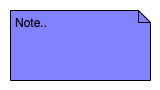
\includegraphics[scale=1.0]{diagram.png}

Aj text môže byť prezentovaný ako obrázok. Stane sa z neho označný plávajúci objekt. Po vytvorení diagramu zrušte znak \texttt{\%} pred príkazom \verb|\includegraphics| označte tento riadok ako komentár (tiež pomocou znaku \texttt{\%}).
\caption{Rozhodujúci argument.}
\label{f:rozhod}
\end{figure*}



\section{Protokoly} \label{ina}

Základným problémom je teda\ldots{} Najprv sa pozrieme na nejaké vysvetlenie (časť~\ref{ina:nejake}), a potom na ešte nejaké (časť~\ref{ina:nejake}).\footnote{Niekedy môžete potrebovať aj poznámku pod čiarou.}

Môže sa zdať, že problém vlastne nejestvuje\cite{Coplien:MPD}, ale bolo dokázané, že to tak nie je~\cite{Czarnecki:Staged, Czarnecki:Progress}. Napriek tomu, aj dnes na webe narazíme na všelijaké pochybné názory\cite{PLP-Framework}. Dôležité veci možno \emph{zdôrazniť kurzívou}.


\subsection{SMTP} \label{ina:nejake}

Niekedy treba uviesť zoznam:

\begin{itemize}
\item jedna vec
\item druhá vec
	\begin{itemize}
	\item x
	\item y
	\end{itemize}
\end{itemize}

Ten istý zoznam, len číslovaný:

\begin{enumerate}
\item jedna vec
\item druhá vec
	\begin{enumerate}
	\item x
	\item y
	\end{enumerate}
\end{enumerate}


\subsection{POP3} \label{ina:este}

\paragraph{Veľmi dôležitá poznámka.}
Niekedy je potrebné nadpisom označiť odsek. Text pokračuje hneď za nadpisom.

\subsection{IMAP} \label{ina:este}

\paragraph{Veľmi dôležitá poznámka.}
Niekedy je potrebné nadpisom označiť odsek. Text pokračuje hneď za nadpisom.

\section{Algoritmus e-mailu} 

\section{Zabezpečenie a filtrácia spamov} 

\section{Súčasná podoba emailu} 

\section{Najpoužívanejšie e-mailové servery} 

\section{Záver} \label{zaver} % prípadne iný variant názvu



%\acknowledgement{Ak niekomu chcete poďakovať\ldots}


% týmto sa generuje zoznam literatúry z obsahu súboru literatura.bib podľa toho, na čo sa v článku odkazujete
\bibliography{literatura}
\bibliographystyle{abbrv} % prípadne alpha, abbrv alebo hociktorý iný
\end{document}
